\chapter{Groundwork\label{chap:groundwork}}

\todo{Figures for this entire chapter have to be rebuilt}

Before implementing any system, it is imperative to understand the data at hand
so as to make correct analytical decisions. In this regard, groundwork was done
to characterize all the input data sources.

\section{Hardware}
The hardware used to produce the results is the Samsung Nexus S (cobranded with
Google) running Android 2.3.4. The official specifications of the device can be
obtained from the manufacturer's website [link to website with reference] A
short listing of the sensors present on the device is given below based on how
the device reports the sensors via the software APIs:

\begin{enumerate}
\item KR3DM 3-axis Accelerometer
\item AK8973 3-axis Magnetic field sensor
\item AK8973 Orientation sensor
\item GP2A Light sensor
\item GP2A Proximity sensor
\item K3G Gyroscope sensor
\item Gravity Sensor
\item Linear Acceleration Sensor
\item Rotation Vector Sensor
\item An 802.11 b/g/n compatible Wifi NIC
\end{enumerate}

It may be noted that of these sensors, the Gravity sensor, the Linear
Acceleration Sensor and the Rotation Vector Sensor are derived sensors. They
depend on filtering the raw data sensed via the accelerometer and the
magnetometer to generate their sensed values. In essence, the Gravity sensor is
a low pass filter over the accelerometer values (since gravity is essentially
stable for the device at a particular orientation), the Linear Acceleration
Sensor is a high pass filter over the accelerometer values (the high frequency
changes in acceleration are presumed to occur due to device motion and thus
correspond to linear acceleration of the device) and the Rotation Vector Sensor
is a composite sensor that fuses Gravity information derived from the
3 axis Accelerometer and the magnetic field information derived from the
3 axis Magnetic field sensor to orient the device in the 3 Dimensional World 
Coordinate space. The actual method used to do so is described in the API
documentation \cite{AndroidSensorManager} and
further discussion is out of scope for this thesis.

\begin{figure}
\centering
    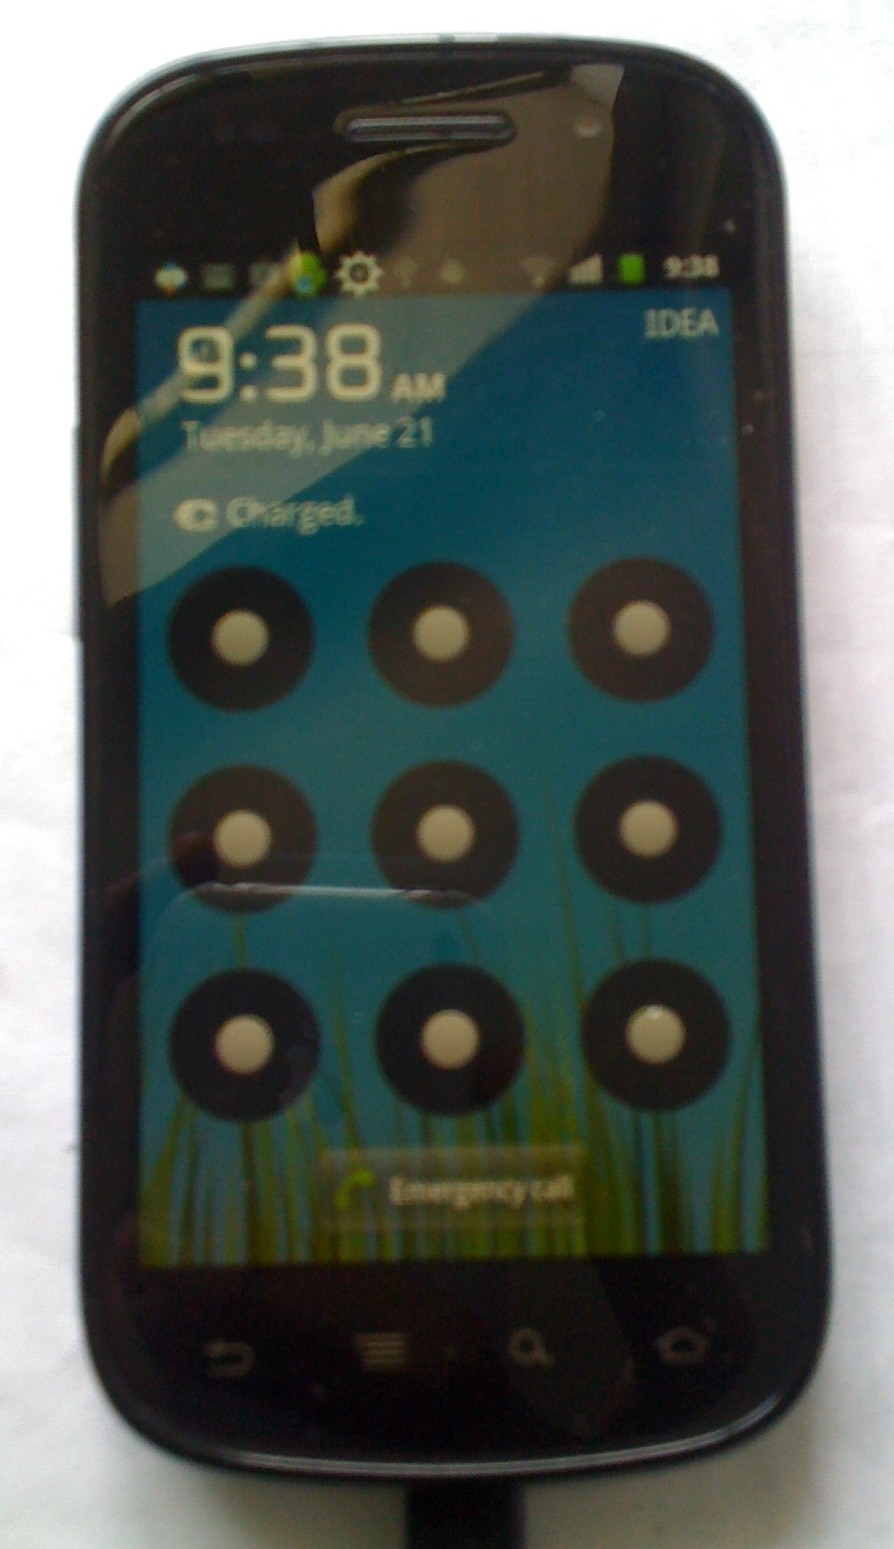
\includegraphics[height=3in]{figures/android_front}
    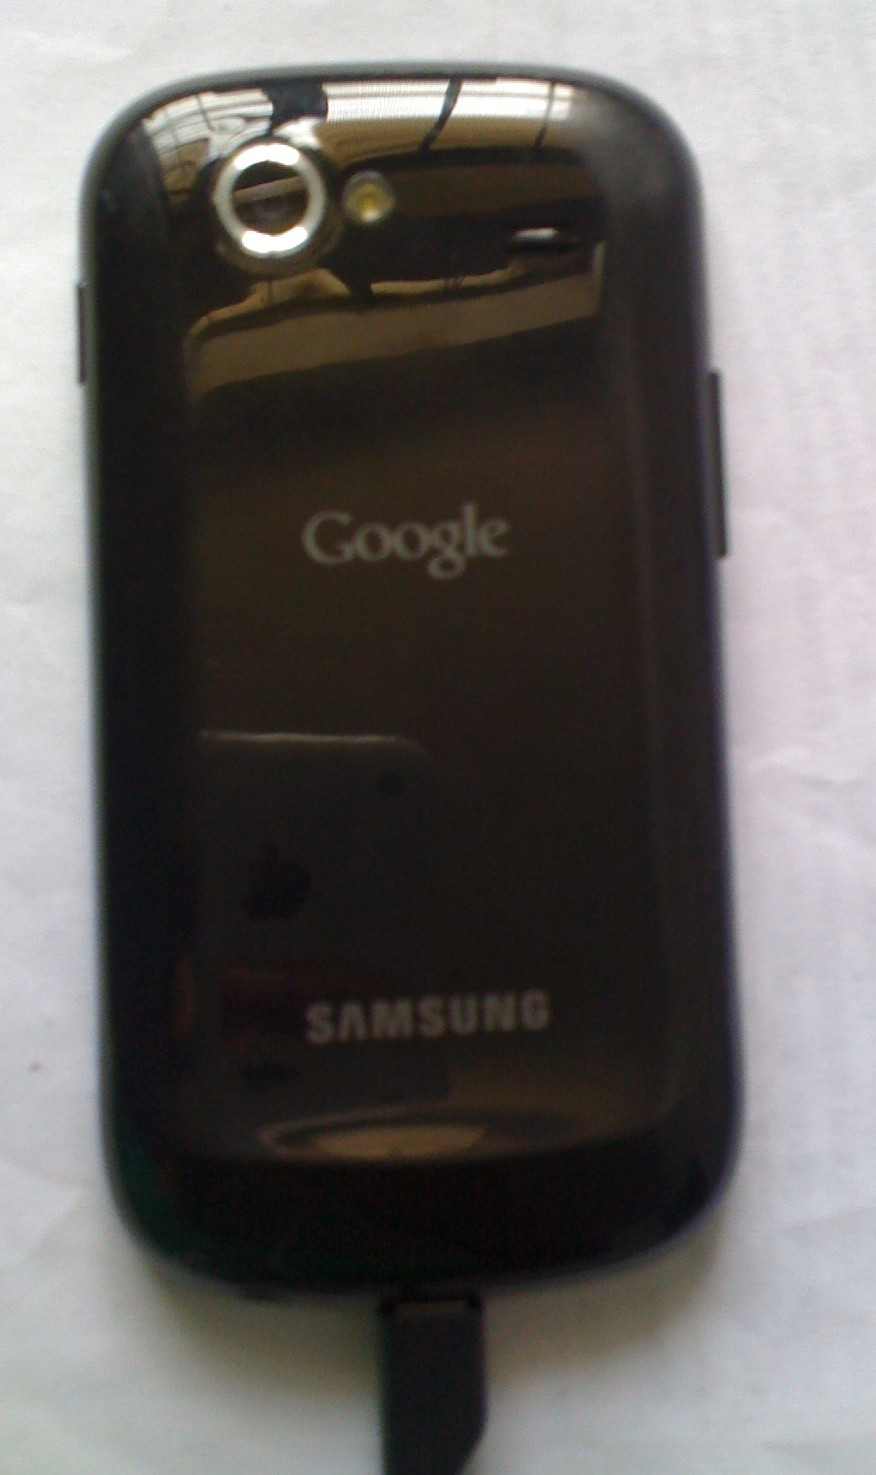
\includegraphics[height=3in]{figures/android_back}
\caption{Google Nexus S manufactured by Samsung}
\end{figure}



\section{Accelerometer}

The MEMS accelerometer on the Nexus S was subject to simple tests to determine 
its noise floor and the degree of separation between signal and noise.
Figure \ref{fig:accel_static} shows a plot of the accelerometer's raw output 
along the Z axis for a stationary device kept on a table. The characteristics
of the accelerometer signal are summarized in Table \ref{tbl:accel_chars}.
As can be clearly observed, the signal degrades while in the palm of a 
user who is standing.

The noise level for the accelerometer was determined to be always less
than $0.6 m/s^2$. The acceleration peaks corresponding to regular walk steps 
usually lie around $2.0 m/s^2$. To allow for a reasonable noise margin and provide
sufficient cushion for additional noise introduced due to the dynamic nature of
walking, we choose a threshold of $1.3 m/s^2$ which is the mean value of the two
peak values. If the absolute value of the Z-axis acceleration sample is less
than this threshold, then the sample will be clamped to zero. For a smartphone
with a similar accelerometer sensor but with different noise characteristics,
the values of the threshold can be varied accordingly. For our purposes, 
the threshold $Q$ is chosen as $1.3 m/s^2$.


\begin{figure}\centering
    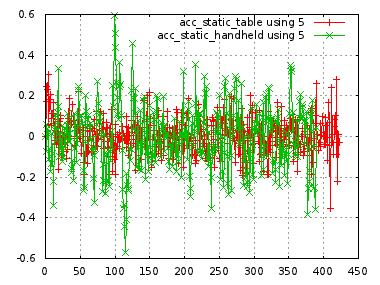
\includegraphics{figures/accel_static.png}
    \caption{Accelerometer Z axis readings when device stationary\label{fig:accel_static}}
\end{figure}

\begin{table}
\centering
\begin{tabular}{c c c c c c c}
\hline
\hline
 & $a_{x,table}$ & $a_{y,table}$ & $a_{z,table}$ & $a_{x,hand-held}$ & $a_{y,hand-held}$ & $a_{z,hand-held}$ \\
\hline
Min & -0.180217 & -0.209914 & -0.352813 & -0.281559 & -0.238432 & \textbf{-0.571722} \\
Median & -0.002995 & 0.001779 & 0.003011 & 0.004029 & -0.005922 & 0.003617 \\
Mean & -0.002065 & -0.002809 & 0.004762 & 0.007291 & -0.003648 & -0.004827 \\
Max & 0.206112 & 0.211490 & 0.306364 & 0.577652 & 0.207061 & \textbf{0.595963} \\
Std. Dev & 0.06985715 & 0.06902411 & 0.08939619 & 0.1100473 & 0.08232208 & \textbf{0.1603238} \\
\hline
\end{tabular}
\caption{Characterization of the Accelerometer (values in $m/s^2$)\label{tbl:accel_chars}}
\end{table}


\section{Magnetometer}

The Nexus S comes with a built in MEMS magnetometer.
It measures the local magnetic field strength in $\mu T$.

In practical tests, the performance is reasonable but the magnetometer has a 
lot of sensor noise and suffers from sensor bias. For example, rotation of 
the smartphone through large angles introduces bias in the readings from the 
magnetometer. Similary, the magnetometer shows a small offset when the device is 
turned through 360 degrees.

Figure \ref{fig:angle_stationary_table}
shows the behaviour of sensor readings under the 2 circumstances when the 
device is on a table and when it is held in the palm of the hand of a user.

\begin{figure}\centering
    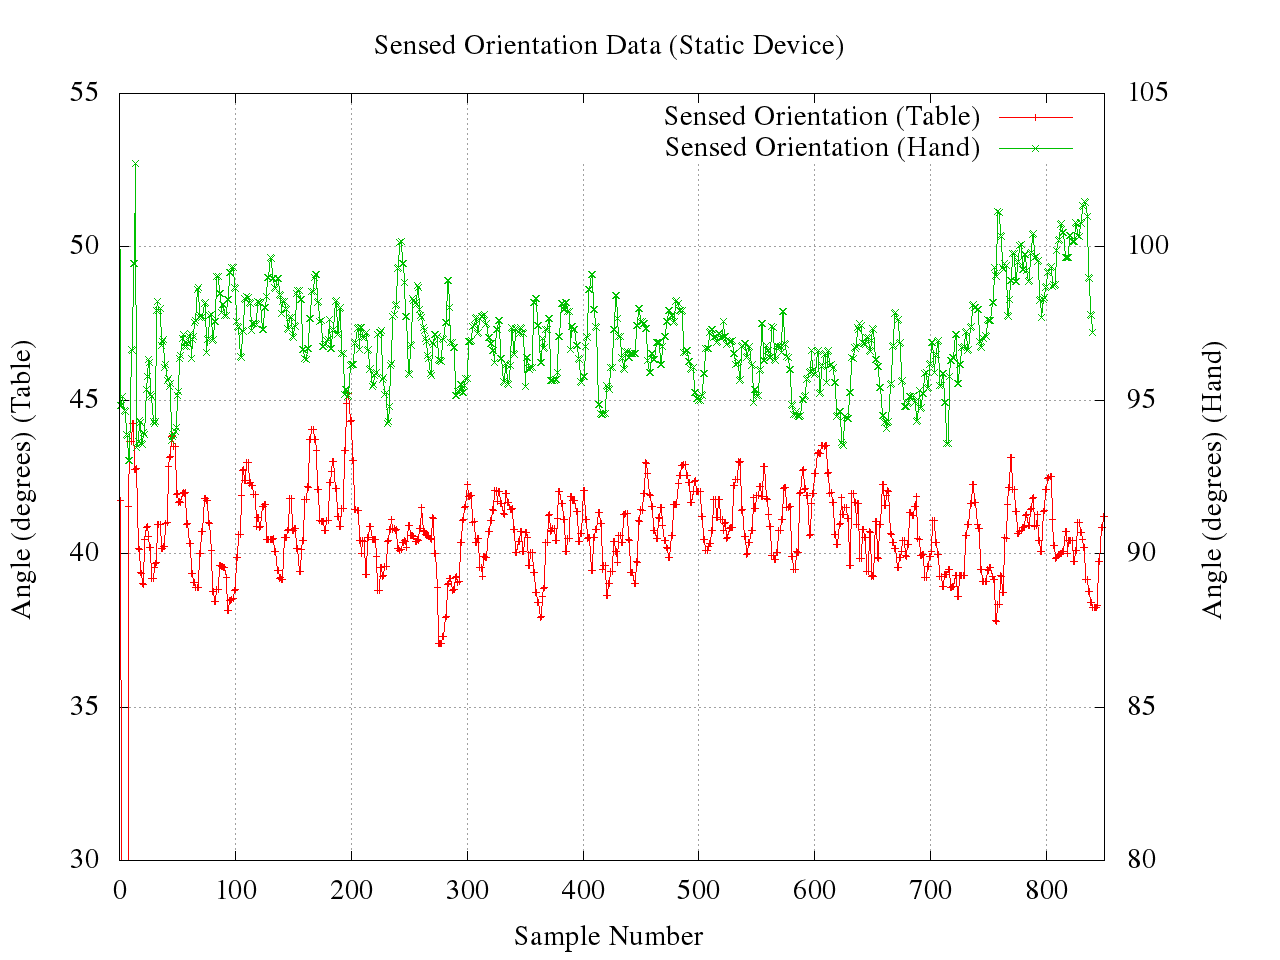
\includegraphics{figures/angle_stationary.png}
    \caption{Derived azimuth angle when smartphone on table\label{fig:angle_stationary_table}}
\end{figure}


\begin{table}
\centering
\begin{tabular}{c c c c}
\hline
\hline
 & $\theta_{table}$ & $\theta_{standing}$ \\
\hline
Maximum Deviation & 8.138436 & 9.688619 \\
Std. Dev. & 1.234318 & 1.521967 \\
\hline
\end{tabular}
\caption{Characteristics of a Stationary Magnetometer (degrees)\label{tbl:angle_chars}}
\end{table}

These values are required to determine choice of parameters for the particle
filter that will be introduced later.

\subsection{Bias study}

Performing rotations in a slow and steady manner yields good results with little
or no bias and sensor lag. See figure \ref{fig:angle_180_rotation_table} which 
shows how the angle measurements behave when the rotated slowly and steadily.
There is only a slight sensor lag and bias visible.

\begin{figure}\centering
    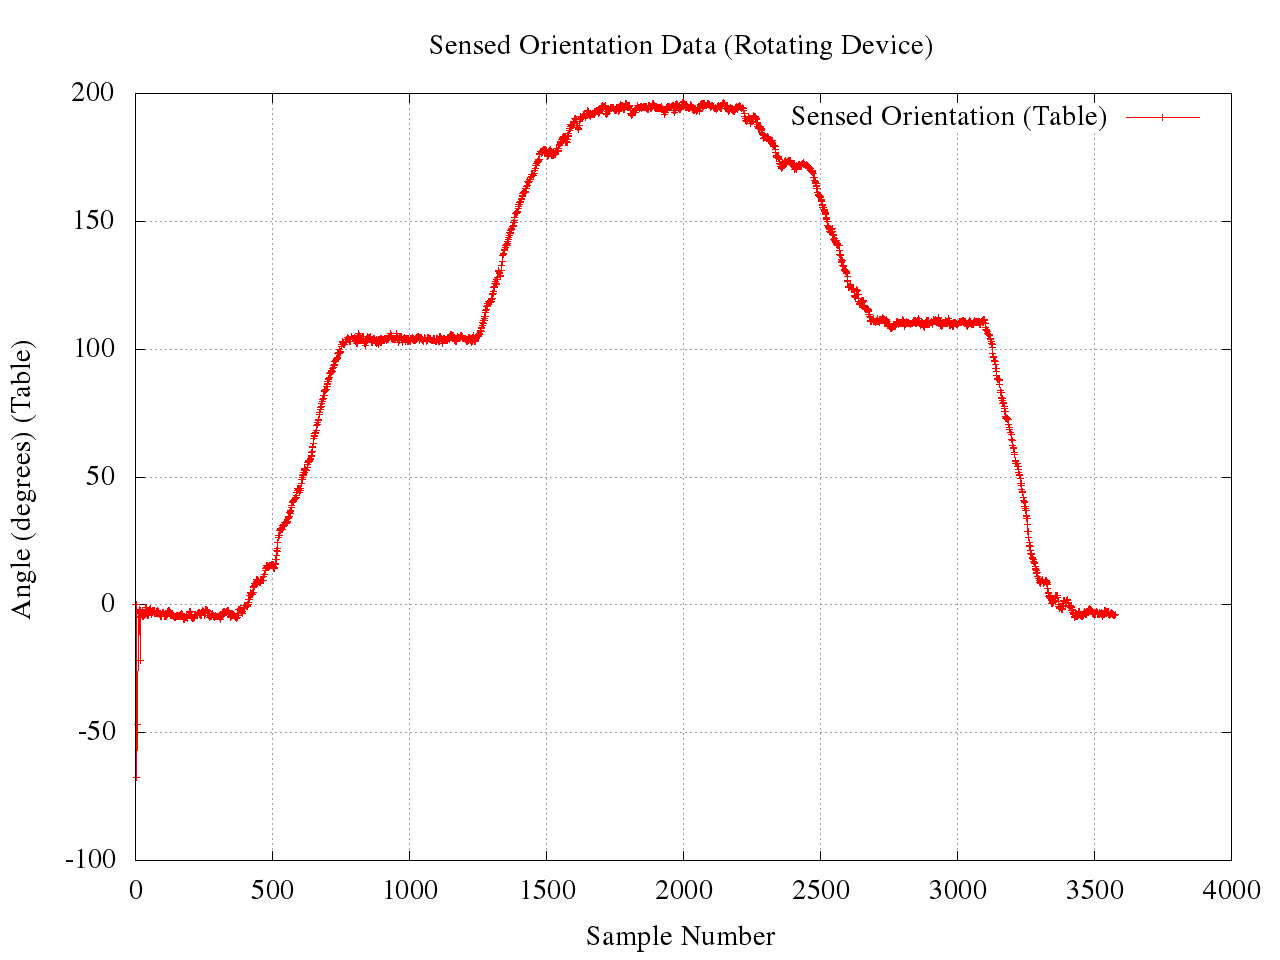
\includegraphics{figures/angle_180_rotation_table.png}
    \caption{Rotation of the phone through 180 degrees (90 degree turns)\label{fig:angle_180_rotation_table}}
\end{figure}


\subsection{Effect of motion}

Although the sensor measurements are stable when the device is on a table,
the measurements go haywire when the device is in a human's hand. See figure
\ref{fig:angle_180_corridoor} - a human is walking along a corridoor and he walks
back. The angle measurements of the return trip are offset by 180 degrees and
the two sets of measurements are compared. You can easily see a large variation
in the angles due to the motion of the human and the dynamic nature of the environment.
Sensor lag and long term sensor value drift is evident in the graph.
This dynamic variation of the measurement of the angle from magnetic north 
introduces error in the inertial navigation system.

\begin{figure}\centering
    \includegraphics{figures/angle_180_corridoor.png}
    \caption{Angle measurements when moving in opp directions.\label{fig:angle_180_corridoor}}
\end{figure}

\begin{table}
\centering
\begin{tabular}{c c c}
\hline
\hline
 & Forward Path & Return Path \\
\hline
Angular Range (Max - Min) & 43.48589 & 32.7897 \\
Standard Deviation & 8.307481 & 5.955799 \\
\hline
\end{tabular}
\caption{Effect of Motion on Orientation Values\label{tbl:angle_motion}}
\end{table}

The values of Table \ref{tbl:angle_motion} indicate the maximum range of 
values over which the angle varies during a walk along a straight corridoor. 
These values are used to set the parameters $\theta_t$ in the algorithm.
The angular range is large but the middle 50\% of the values lie 
between 11 to 13 degrees apart which corresponds with the standard deviation
values measured.

\section{Test Environment\label{sec:test_environment}}

The location chosen for performing all experimental verification of the
proposed work was Floor 3, Wing 7 and 8 of Ravindra Bhawan at the IIT Roorkee
campus. The environment is suitable for this purpose due to a number of reasons:

\begin{enumerate}
\item There are a large number of Wifi Access Points in close proximity 
    installed on the premises.
\item Wifi Access Points of neighbouring wings and floors provide diversity
    to the location fingerprints.
\item Long corridoors of around 30-32 metres each provide long stretches of
    similar environment for evaluation of algorithm performance over larger
    distances.
\end{enumerate}

A map of the location is shown in Figure \ref{fig:ravindra_map}. The red lines
indicate walls, blue lines indicate windows and green lines indicate doors.
Wifi Access Points are marked with stars on the map. This map has been used
for all the experiments detailed below and while determining the results as 
stated in Chapter \ref{chap:results}.

\begin{figure}
    \centering
    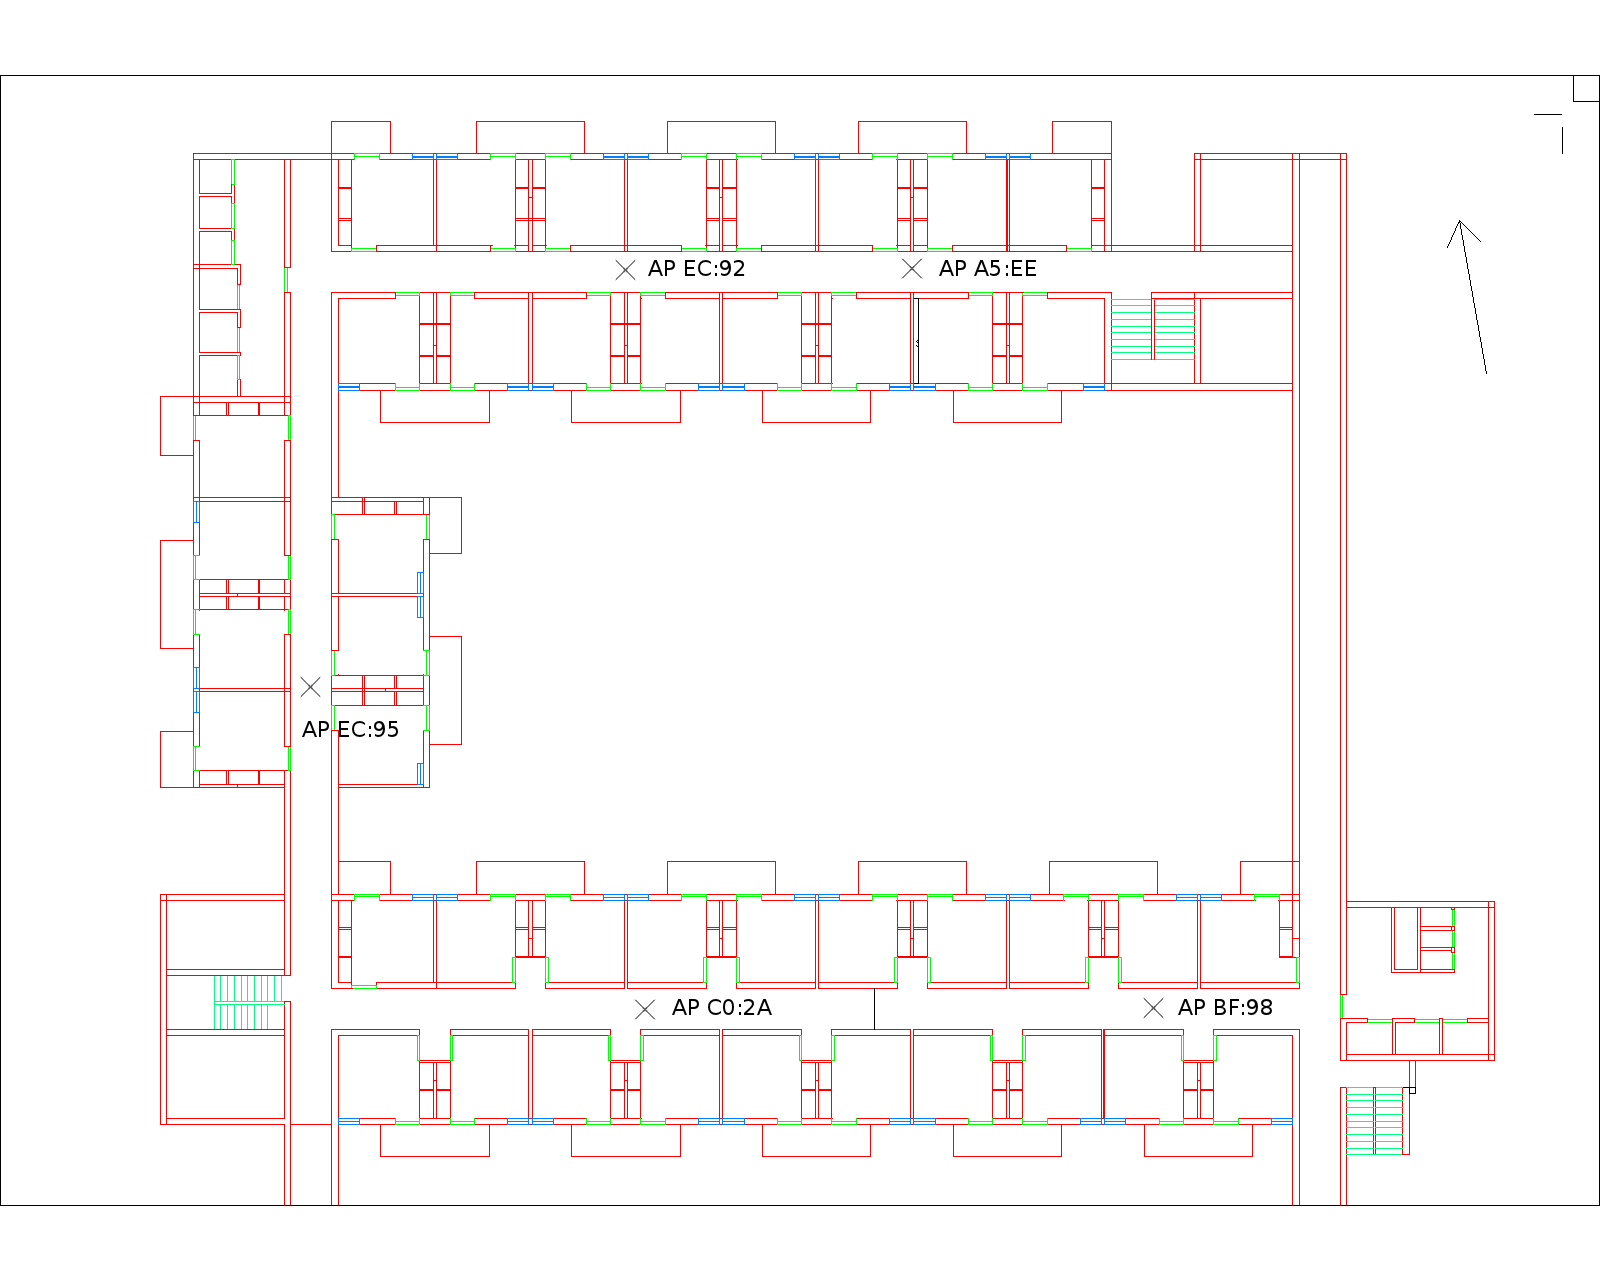
\includegraphics[width=5in]{figures/ravindra_map_ap.png}
    \caption{A map of the experimental environment\label{fig:ravindra_map}}
\end{figure}


\section{Wifi Signal Strength Distribution}

Wifi signals are used in our proposed system during the recovery process.
Other systems and the control algorithms use Wifi for correcting positioning
drift. Hence, it is important to understand the strengths and limitations of 
Wifi based positioning. In order to do so, we need to first characterize
the Wifi signal.

The behaviour of the wifi signal strength distribution for a stationary laptop 
and smartphone was analyzed to characterize the input wifi signal.

\subsubsection{Short term duration}

Figure \ref{fig:closestAPshortterm} shows the variation of signal strength of 
AP EC:95 for a smartphone placed within a room in a 
Non-Line Of Sight configuration.

\begin{figure}\centering
    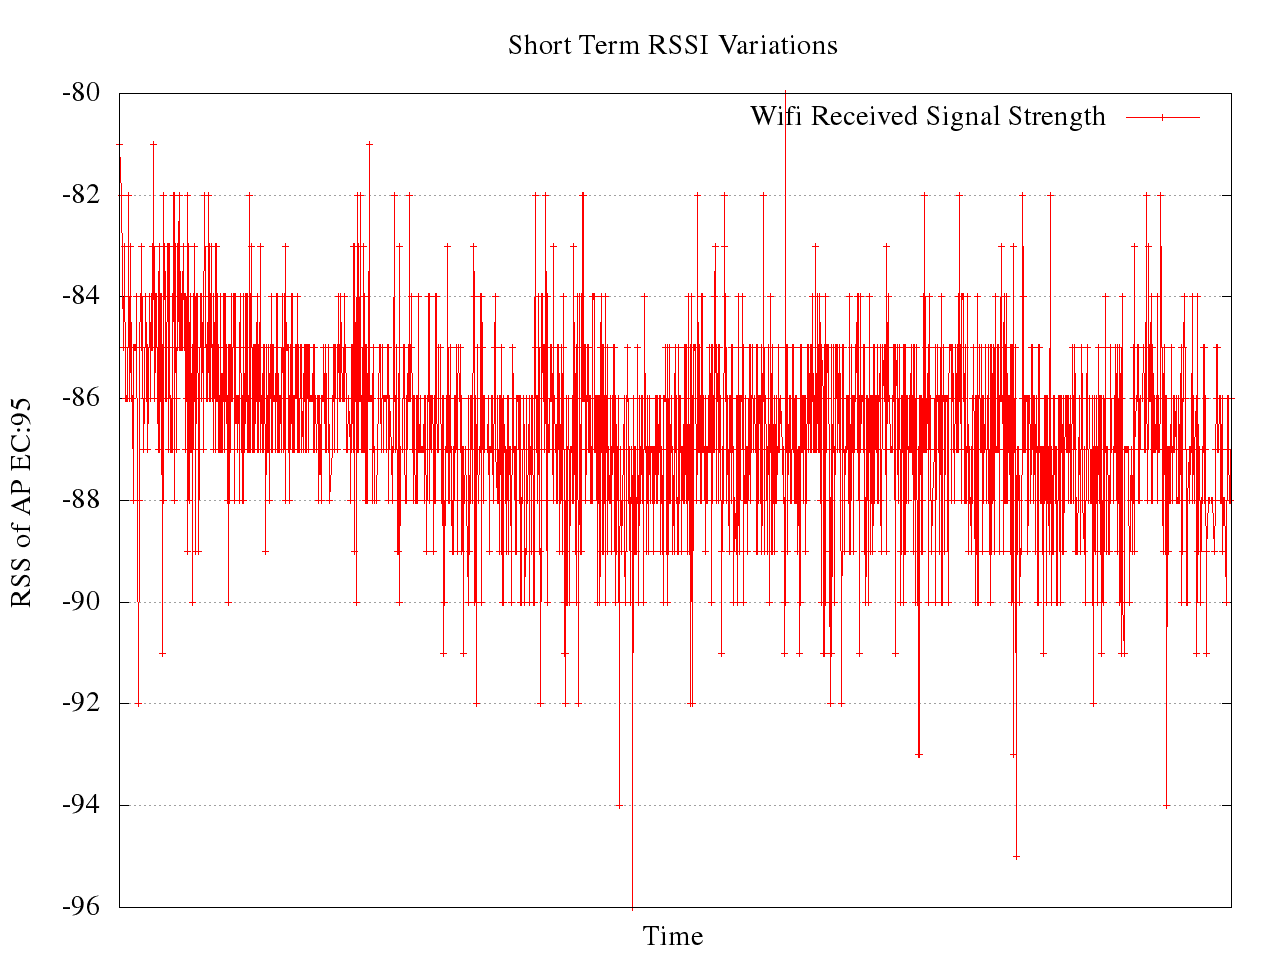
\includegraphics{figures/wifi_short_term.png}
    \caption{Variation of RSSI for AP EC:92 \label{fig:closestAPshortterm}}
\end{figure}

\subsection{7 day study}

The Wifi Access Point RSSI values were monitored over a 7 day period 
(Jan 5 2011 - Jan 13 2011) from room S-152 and the resulting signal strength 
data was analyzed.

\pdfimageresolution 72

\begin{figure}\centering
    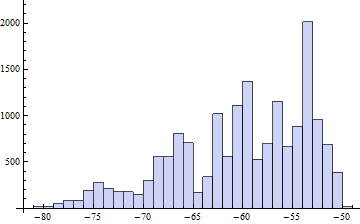
\includegraphics{figures/histogram_00_1C_F0_CB_EC_92.png}
    \caption{Distribution of RSSI values AP EC:92\label{fig:histogram_00_1C_F0_CB_EC_92}}
\end{figure}

As you can see in Figure \ref{fig:histogram_00_1C_F0_CB_EC_92}, the signal 
strength distribution for the closest access point is highly non-gaussian. This
concurs with the conclusions of Kaemarungsi and Krishnamurthy in \cite{KStats}.

\begin{figure}\centering
    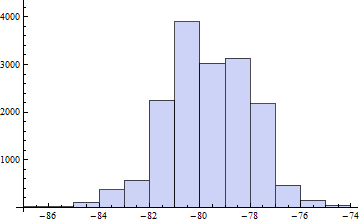
\includegraphics{figures/histogram_00_1C_F0_CB_EC_95.png}
    \caption{Distribution of RSSI values AP EC:95\label{fig:histogram_00_1C_F0_CB_EC_95}}
\end{figure}

\begin{figure}\centering
    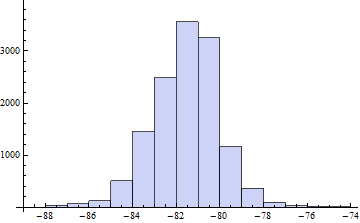
\includegraphics{figures/histogram_00_19_5B_77_A5_EE.png}
    \caption{Distribution of RSSI values for the AP A5:EE\label{fig:histogram_00_19_5B_77_A5_EE}}
\end{figure}

\pdfimageresolution 300

\begin{figure}\centering
    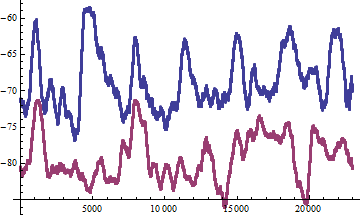
\includegraphics{figures/moving_average.png}
    \caption{3 hour moving average of RSSI values for the 7 day survey\label{fig:moving_average}}
\end{figure}

In contrast, Figure \ref{fig:histogram_00_19_5B_77_A5_EE} doesn't show such a 
pronounced non-gaussian nature whereas 
Figure \ref{fig:histogram_00_1C_F0_CB_EC_95} shows more leanings towards a
non-gaussian distribution.

Table \ref{tbl:wifi_signal_analysis} states the features of the signal with 
respect to 3 different APs. However, this table does not state the entire 
story. 

Figure \ref{fig:moving_average} is the time domain plot of the signal strength
samples smoothed as a moving average over 300 samples as received by a fixed 
location. It is quite evident that the variations in the signal strength 
are highly localized with significant peaks and valleys. Plots for other APs
show this kind of clustering behaviour too but to a lower extent. 
Given the uncorrelated nature of wifi signals, it is highly likely that 
signal variations will not move in a correlated fashion and thus even 
location fingerprinting based systems will find it very difficult to 
create a distance function that will be able to estimate the location of a
device reliably from the RSSI values given that the survey database will 
always be subsampling the signal. 

Thus it is quite evident that the input wifi signal is a highly noisy and
unreliable source of information.


\begin{table}
\centering
\begin{tabular}{c c c c c c c c c}
\hline
\hline
 & Min & $1^{st}$ quartile & Median & Mean & $3^{rd}$ quartile & Max & NA & SD\\
\hline
AP EC:92 & -82.00 & -66.00 & -60.00 & -60.62 & -55.00 & -49.00 & 27.36\% & 6.638592\\
AP EC:95 & -87.00 & -81.00 & -80.00 & -80.16 & -79.00 & -74.00 & 30.64\% & 1.691343\\
AP A5:EE & -89.00 & -83.00 & -82.00 & -82.05 & -81.00 & -73.00 & 43.48\% & 1.580761\\
\hline
\end{tabular}
\caption{Wifi Signal Analysis\label{tbl:wifi_signal_analysis}}
\end{table}

\section{Effect of motion on signal strengths}

To analyze the effect of motion on the RSSI values from the APs, a simple walking
test was done along a corridoor. The variation of RSSI values seen from the AP in
the corridoor is shown in \ref{fig:wifi_corridoor_walk}.

\begin{figure}\centering
    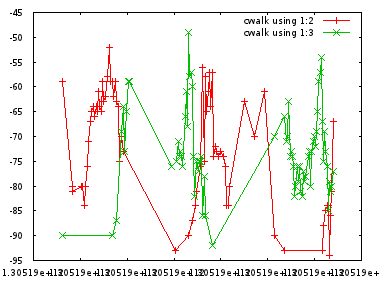
\includegraphics{figures/wifi_corridoor_walk.png}
    \caption{AP EC:95 RSSI: Walk up and down the corridoor\label{fig:wifi_corridoor_walk}}
\end{figure}


\subsection{Inferences}
From the figure, it can be clearly seen that orientation with respect to 
AP is important. There is significant noise in the signal even though the AP 
is in the line of sight. Thus retaining orientation data with respect to 
an AP is an important criteria while surveying the test environment to 
collect location fingerprints.

\section{Generating a Location Fingerprinting Dataset}

A Wifi Survey was carried out in the test environment to generate a location 
fingerprint dataset. To ensure uniform sampling of the environment, 
a $1m \times 1m$ grid was set up on the ground and Wifi RSSI readings were taken 
at 8 different orientations per point on the floor. 
Figure \ref{fig:grid_pic} shows a snapshot of a small area of the test environment.
Grid points have been marked out on the floor. 
Wifi RSSI samples were taken at these grid points along 8 different orientation 
values. Some samples, however, could not be taken due to obstructions 
present at the site.

\begin{figure}
    \centering
    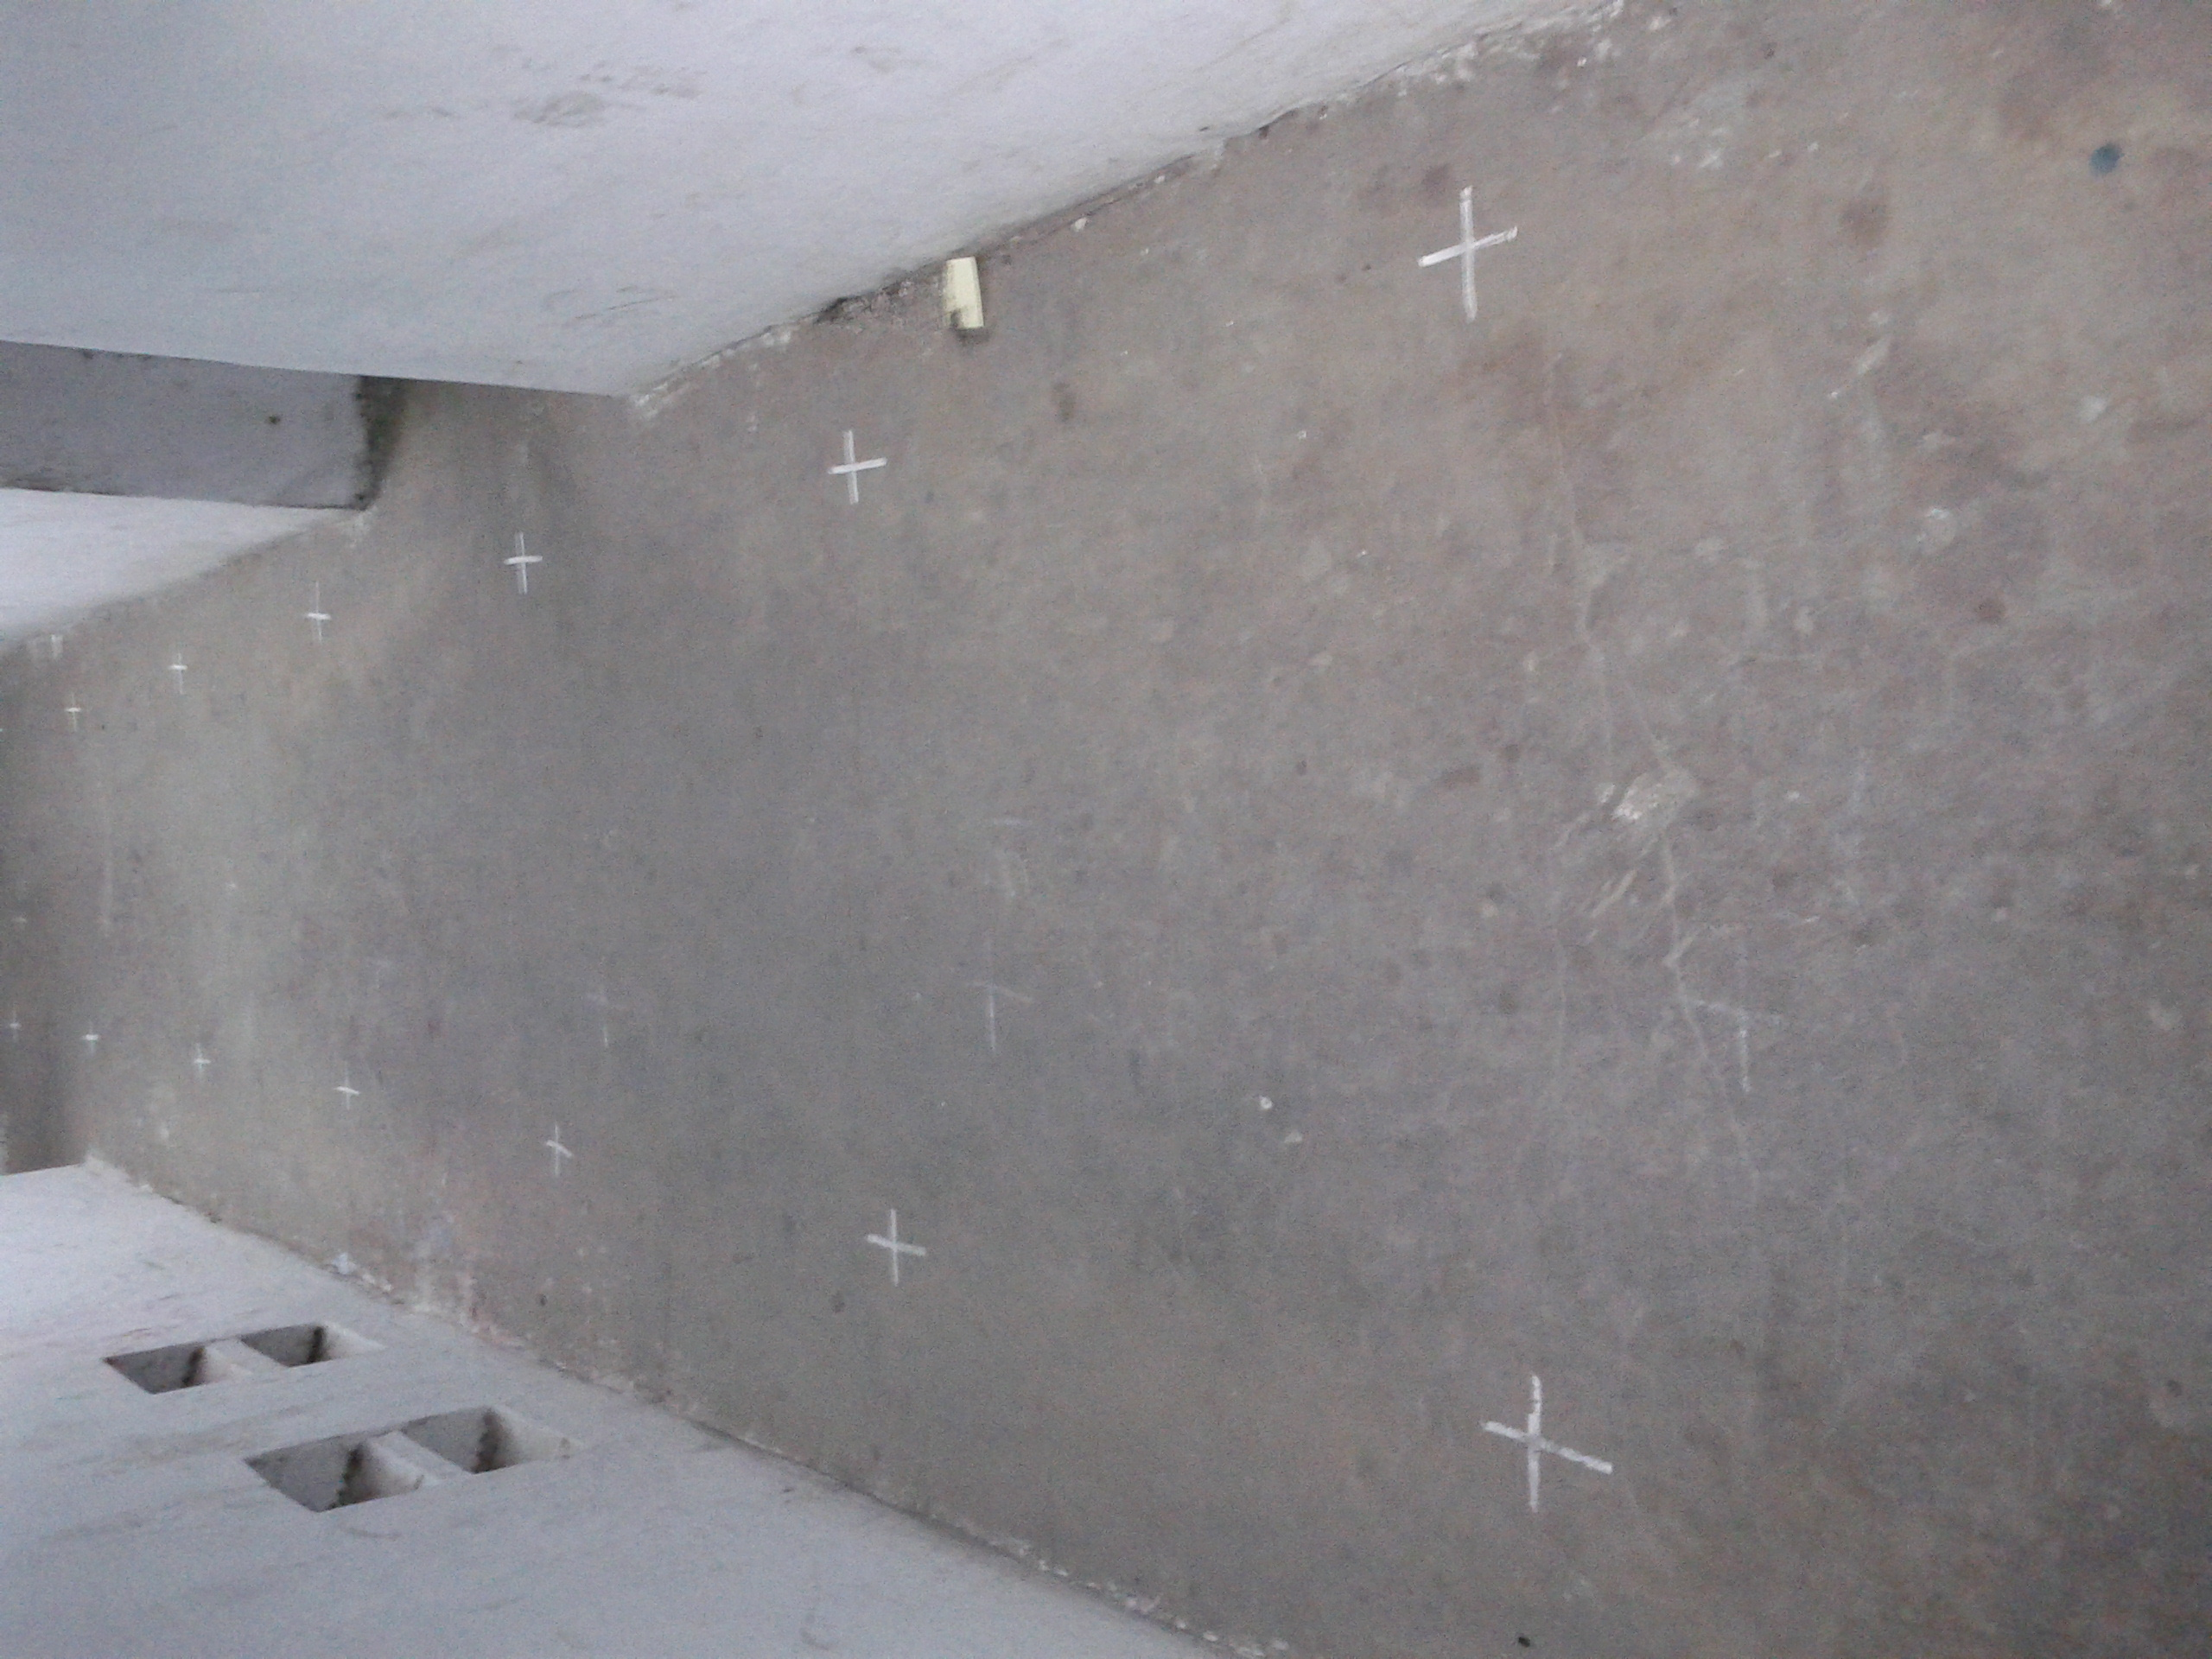
\includegraphics[width=5in,angle=270]{figures/grid_pic}
    \caption{Picture of the $1m \times 1m$ grid drawn on the floor\label{fig:grid_pic}}
\end{figure}

\section{Testing Wifi Positioning Accuracy using KNN\label{sec:knn_pos}}

A KNN based location system was implemented to test location accuracy for positioning using Wifi Signal Strengths. 
This was work done as part of the Masters project in the same test location. 
The results of the project are included here. Although the project was 
done using a laptop instead of a smartphone and with a different set of survey data, 
it is expected that the results will be comparable as the test environment was the same.

\begin{table}[h]
    \centering
    \caption{Performance of KNN based indoor positioning system \label{tab:knnperf}}
    \begin{tabular}{|l|c|c|c|}
    \hline
              & Mean Error $\bar{e}$ (m) & $\sigma_{error}$ (m) & $\bar{e} + 2 \sigma_{error}$ \\
    \hline
    \hline
    $K = 1$    & 2.8 & 2.7 & 8.2 \\
    $K = 2$    & 2.8 & 2.7 & 8.2 \\
    $K = 3$    & 2.7 & 2.7 & 8.1 \\
    $K = 4$    & 2.3 & 2.8 & 7.9 \\
    \hline
    \end{tabular}

\end{table}

\section{Summary}

To conclude, we can state that by doing all the experiments and other 
ground-work mentioned in this chapter, we have obtained a fair idea 
about the inputs of the system and various system parameters required
for the algorithms. The groundwork thus helps in guiding the implementation of
the system. Since groundwork was being done in conjunction with algorithm
design, some feedback from the groundwork was also incorporated into improving
the design of the proposed method of Chapter \ref{chap:proposed_method}.

By doing the groundwork, we have been able to derive the ranges of parameters of 
the proposed algorithm. These ranges are listed in Table \ref{tbl:algo_params}.

\begin{table}
\centering
\begin{tabular}{c c}
\hline
\hline
Parameter & Value\\
\hline
For Noise Filtering & \\
Threshold $T$ & $> 0.352813$\\
Threshold $Q$ & $Q > 0.595963$ and $Q < 2.0$\\
\hline
For Orientation Bias & \\
$\sigma_{angle}$ & 8.307481 degrees\\
\hline
For NN based positioning & \\
Wifi Orientation Tolerance & $> 43.48589$ degrees\\
Wifi Positioning Error & $> 2.8 m$ with S.D. $> 2.7 m$\\
\hline
\end{tabular}
\caption{Algorithm Parameters Determined by Ground Work\label{tbl:algo_params}}
\end{table}
